\section{Regression}
\begin{itemize}
	\item Optimal solution for regression $\arg\min_f\E(Y - f(X))^2$ given by $f^*(x) = \E(Y \mid X=x)$ \\
		However, $\P(Y\mid X)$ and $\P(X)$ are unknown
	\item \textbf{(Parametric) maximum likelihood: }
	\begin{enumerate}
		\item Assume $Y\mid X \sim \mathcal N(f(X), \sigma^2\mathbf I)$
		\item Solve $\arg\max_f\sum_{i = 1}^n \log\P(Y = y_i\mid X=x_i, \sigma^2)$
	\end{enumerate}
	\item \textbf{Statistical learning theory: } \\ Directly minimize empirical risk $\arg\min_f\sum_{i = 1}^n (y_i - f(x_i))^2$
\end{itemize}
\subsection{Linear Regression}
$$
	Y = \beta_0 + \sum_{j = 1}^d X_j\beta_j = X^T\beta, Y\in \mathbb R
$$
\text{$\beta_0$ is called bias, $X,\beta \in \mathbb R^{d+1}$.}


Ordinary least squares regression model: least-squares cost function. 
\begin{itemize}
	\item[$\Rightarrow$] Minimization either through gradient descent or closed form solution 
\end{itemize}
\subsubsection{Residual Sum of Squares (RSS)}

$
	RSS(\beta) = \sum_{i = 1}^n (y_i - x_i^T\beta) = (\mathbf y - \mathbf X\beta)^T(\mathbf y - \mathbf X\beta)
$

$\nabla_\beta RSS(\beta) = 0 \implies \hat\beta = (\mathbf{X^TX})^{-1}\mathbf X^T\mathbf y$


\subsubsection{Prediction}
$$
	\hat{\mathbf y} = \mathbf X \hat\beta = \mathbf X(\mathbf X^T\mathbf X)^{-1}\mathbf X^T \mathbf y, 
$$
where $\mathbf X(\mathbf X^T\mathbf X)^{-1}\mathbf X^T$ is an orthogonal projectin on the space spanned by the columns of $\mathbf X$.

\begin{itemize}
	\item Assume additive gaussian noise: $Y = \beta_0 + \sum_{j = 1}^d X_j\beta_j + \epsilon = X^T\beta + \epsilon $ with conditional mean $\E(Y\mid X_1, ..., x_d) = X^T\beta$
	\item Distribution: $\hat \beta \sim \mathcal N(\beta, (\mathbf X^T\mathbf X)^{-1}\sigma^2)$
\end{itemize}

\subsubsection{Local weighting}
We can add weights to the features, such that not all of them are treated equally:
\begin{equation*}
	\hat\beta = \argmin_\beta \sum_i w_i (y_i - \transp{x_i}\beta)^2 
\end{equation*}

If $w_i$ is large, this feature will become very important, if $w_i$ is small it will be pretty much ignored.

Predict: $y = x\beta$


\subsection{Bias / Variance Dilemma}
Goal: Minimize bias and variance simultaneously (usually impossible).
\begin{itemize}
	\item Data $D = \{(x_i, y_i)_{i = 1}^n\}, y_i\in \mathbb R$
	\item Objective: Find regression function $f\in \mathcal C$ such that $\E( Y - f(X))^2$ is minimal.
	\item Optimum $f^*(x) = \E(Y \mid X=x)$
	\item Estimator $\hat f(X)$ depends on random variable $X$ and data $\mathcal D$
	\item \textbf{Problems: } we only have a finite training set, and the complexity of hypothesis class $\mathcal C$ is unknown.
\end{itemize}

\vspace{1em}
\textbf{Tradeoff: }
\begin{itemize}
	\item Small data sets and large $\mathcal C$: Variance large, bias small
	\item Large data set, small $\mathcal C$: Variance small, bias large
\end{itemize}
\textit{The optimal tradeoff between bias and variance is achieved when we avoid both underfitting (large bias) and overfitting (large variance)}

\vspace{1em}
\textbf{Prediction error: }
\begin{align*}
		\E_D\E_{Y\mid X=x}\left(\hat f(x) - Y\right)^2 &=\\
	(\text{variance})\quad &\E_D(\hat f(x) - \E_D(\hat f(x))^2 \\
	(\text{bias$^2$})\quad &+ \left(\E_D(\hat f(x)) - \E(Y\mid X=x)\right)^2 \\
	(\text{noise})\quad &+  \E(Y - \E(Y\mid X=x))^2
\end{align*}

\subsection{Overfitting}
\begin{itemize}
	\item \textbf{Regularization}: Add model complexity term to cost function 
	$\arg\min_\theta\sumi n l(f(x_i, \theta, y_i) + R(\theta) $\\
	Often equivalent to choosing a prior in a bayesian framework and using a MAP estimator.
	\item Model selection based on \textbf{generalization error estimate} (e.g. cross-validation)
	\item \textbf{Ensembles} of classifiers (See Section 9)
\end{itemize}



\subsection{Ridge Regression, LASSO}
\begin{center}
{\footnotesize
	\begin{tabular}{ p{0.1\columnwidth} | p{0.39\columnwidth} | p{0.39\columnwidth} } 
		& \textbf{Ridge Regression} & \textbf{LASSO}\\\hline
			
		Reg. $R$ & $\lambda\beta^T\beta$ & $\lambda\norm{\beta}_1$ \\\hline
		Bay. view: & $Y | (X, \beta) \sim$ $\mathcal N(x^T\beta, \sigma^2\mathbf I)$, 
		
		prior $\beta: \beta\sim\mathcal N(0, \sigma^2 / \lambda\mathbb I)$ & 
			$Y | (X, \beta) \sim$ $\mathcal N(x^T\beta, \sigma^2\mathbf I)$, Laplace prior:
			
			 $p(\beta_i) = \frac{\lambda}{4\sigma^2}\exp(-|\beta|\frac{\lambda}{2\sigma^2})$
		\\\hline
		Solution & $\hat\beta_\lambda^{\textit{ridge}} = (\mathbf X^T\mathbf X + \lambda\mathbf I)^{-1}\mathbf X^T\mathbf y$ & Optimization techniques 
		
			(e.g. LARS), $\norm{\beta}_1$ is not differentiable. \\\hline
	\end{tabular}
	}
\end{center}

\subsubsection{Singular Value Decomposition}
\begin{itemize}
	\item Take centered $X$ and perform SVD: $X = UDV^T$ ($U, V$ have orthonormal columns)
	\item SVD of least squares fitted vector: 
	
	$\X\hat\beta^{ls} = \X(\X^T\X)^{-1}\X^T\y = \mathbf U \mathbf U^T\y$
\end{itemize}

\subsubsection{Ridge regression: }
If the $\beta_j$ are unconstrained, they can explode (high variance). We can \textbf{control the variance by regularizing the coefficients: }

\vspace{1em}
\textbf{Constraint: }
\begin{align*}
	&\min \sumi n(y_i - \transp{\beta}x_i)^2 \textit{ s.t. } \sumj d \beta_j^2 \leq t \\
	\iff &\min \transp{(y- \X\beta)}(y-\X\beta)  \textit{ s.t. } \sumj d \beta_j^2 \leq t \\
	&\textit{Assume $\X$ standardized, $\y$  centered}
\end{align*}
We can rewrite this as
\begin{align*}
	\mathit{PRSS}(\beta)_{l_2} 	&= \sumi n(y_i - \transp{x_i}\beta)^2 + \lambda\sumj d \beta_j^2 \\
								&= (\y - \X\beta)^\top(\y - \X\beta) + \lambda\norm{\beta}^2
\end{align*}

\begin{align*}
	\X\hat\beta^{\text{ridge}} &= \X(\X^T\X + \lambda\mathbf I)^{-1}\X^T\y \\
	&= \mathbf{UD} (\mathbf D^2 + \lambda \mathbf I)^{-1}\mathbf{DU}^T\y \\
	&= \sumi d \mathbf u_j  \frac{d_{j}^2}{d_{j}^2 + \lambda} \mathbf u_{j}^T\mathbf y 
\end{align*}



$\frac{d_j^2}{d_j^2 + \lambda}$ is small for small singular values $d_j$ and goes to 1 for large SV. This suppresses contributions of small eigenvalues.
\begin{itemize}
	\item $\hat \beta^\textit{ls} = \beta + (\textit{Inflammation term dep. on $\inv{\Sigma}$}) \epsilon$ (\href{https://kunyu-he.com/2020/01/11/SVD-in-Machine-Learning-Ridge-Regression-and-Multicollinearity/}{Derivation})
	\item With multicollinearity (i.e. columns of $\X$ are not independent), some $d_i, d_j$ will be close to 0. The diagonal element $1/d_j$ will then be huge. 
	\item This leads to large inflammation term and therefore \textbf{great deviation in the least squares weights from the true weights.}
	\item Ridge regression projects $\y$ onto the components with large $d_j$
	\item This shrinks the coefficients of low-variance components.
\end{itemize}

\subsubsection{The LASSO (Least Absolute Shrinkage and Selection Operator)}
\begin{align*}
	\hat\beta^{\text{LASSO}}  	&= \argmin_\beta \sumi n(y_i- \beta_0 - \sumj d x_{i,j}\beta_j)^2 \\
								&= \argmin_\beta (\y - \X\beta)^\top(\y-\X\beta)\\
	&\text{subject to} \sumj d|\beta_j| \leq s.
\end{align*}

We can rewrite this as
\begin{align*}
	\mathit{PRSS}(\beta)_{l_1} 	&= \sumi n(y_i - \transp{x_i}\beta)^2 + \lambda\sumj d |\beta_j| \\
								&= (\y - \X\beta)^\top(\y - \X\beta) + \lambda|\beta_j|
\end{align*}

\textit{LASSO estimates are known to be sparse with few coefficients non-vanishing (Reason: LSE error surface hits the corners of the constraint surface often).
}
\begin{center}
	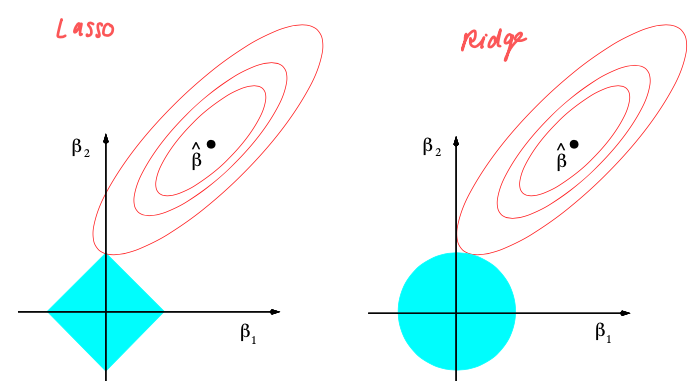
\includegraphics[width=0.8\columnwidth]{images/4-ridge-vs-lasso}\\
	\textit{Contours of error and constraint functions. Blue = constraint regions, red=contours of least squares error function.}
\end{center}
\begin{itemize}
	\item Often, we believe that some $\beta_j$ should be $0$.
	\item Large $\lambda$ will set some coefficients equal to $0$ $\to$ sparse solution
	\item \textbf{LASSO will perform model selection for us}
\end{itemize}


\subsection{nonlinear regression with basis expansion}
\textbf{Idea: } Transform variables $X$ nonlinearly and fit a linear model in the resulting feature space.

\begin{equation*}
	\begin{gathered}			
		f(X) = \sum_{m=1}^M \beta_mh_m(X) \\
		h_m(X) : \R^d\mapsto \R, 1\leq m \leq M
	\end{gathered}
\end{equation*}

\textbf{Smoothing Splines:}	
Cubic splines are a common choice for $h$.
\begin{itemize}
	\item Know selection: Use the maximal number of knots and control the smoothness by regularization:
	$$
		RSS(f, \lambda) = \sumi n(y_i - f(x_i))^2 + \lambda\int(f''(x))^2 dx
	$$
\end{itemize}

\subsection{Regression with Wavelets}
Many phenomena are local perturbations (e.g. face muscles) and can hence be modeled by wavelets (?).

Haar wavelet, symmlet-8 wavelet, denoising by wavelet shrinkage
